% AR-Politeia Cycle 1 -- Nature-format journal draft.
% Generated by the isolated journal_nature writing node.
% Source of truth: research/orchestration/comprehensive.json,
% research/findings.json, rules/journal-formats.md.
%
% STATUS: internal draft, not for external submission. Cycle 1 does not
% support a positive Nature claim (see Table 1 and claims.json).
\documentclass[11pt]{article}

\usepackage[T1]{fontenc}
\usepackage[utf8]{inputenc}
\usepackage{amsmath,amssymb}
\usepackage{booktabs}
\usepackage{graphicx}
\usepackage{xcolor}
\usepackage{tikz}
\usetikzlibrary{arrows.meta,positioning,calc,fit,backgrounds}
\usepackage[margin=1in]{geometry}
\usepackage[colorlinks=true,linkcolor=blue!60!black,citecolor=blue!60!black,urlcolor=blue!60!black]{hyperref}
\usepackage{caption}
\usepackage{microtype}

\definecolor{accent}{RGB}{20,72,130}
\definecolor{warn}{RGB}{160,40,40}
\definecolor{ok}{RGB}{20,120,70}

\newcommand{\code}[1]{\texttt{#1}}

\title{\bfseries A numerical-calibration gate halts a preregistered test of whether resource arrangement shapes socioeconomic structure}
\author{AutoResearcher Project \code{ar-politeia}, Cycle 1}
\date{Internal draft -- 2026-08-21}

\begin{document}
\maketitle

\begin{abstract}
Spatial heterogeneity of resources is widely assumed to influence how populations
aggregate and how wealth is distributed, but separating the effect of resource
\emph{arrangement} from resource abundance is difficult in observational data.
Here we report a preregistered, generative-model test designed to hold total
resources, resource histogram, accessible area, population, and initial wealth
matched while contrasting a clustered resource landscape with its exact pixel
shuffle. The test did not reach the scientific comparison. In a minimal
fixed-population Langevin model with two terrain channels and symmetric wealth
exchange, the conservation, non-negativity, and equal-state absorption checks
passed, but the preregistered numerical-calibration gate failed on
time-step convergence and stationarity. Consequently, the confirmatory
landscape, channel-ablation, and robustness experiments were blocked before any
scientific outcome was produced. Cycle 1 therefore supports no confirmatory
claim; its main result is a reproducible numerical boundary that must be crossed
before landscape effects can be interpreted causally.
\end{abstract}

\vspace{1.4em}
\noindent\textbf{Status.} This is an internal journal-format draft. The
project's comprehensive record explicitly recommends \emph{not} submitting a
journal version in Cycle 1 because the calibration gate failed. The manuscript
is retained as the Nature-format condensation of that record; every numerical
statement below is traceable to \code{research/findings.json} and
\code{research/orchestration/comprehensive.json}.

\medskip
\noindent
The question of whether the physical environment or human institutions drive
long-run differences in settlement and inequality has broad scientific
resonance. A cleaner causal version of that question is narrower: once the
total amount of resource and its statistical distribution are fixed, does the
\emph{spatial autocorrelation} of the resource field still change where people
gather and how wealth is distributed? If it does, then spatial arrangement is a
causal ingredient in socioeconomic structure. If it does not, then models can
ignore arrangement and retain only marginal resource statistics. Answering this
question requires a controlled comparison: a clustered landscape and a
spatially shuffled landscape with the same pixel values, the same total
resource, the same accessible area, and the same initial conditions. Any
difference between them can then be attributed to spatial organization rather
than to a hidden abundance or histogram confound.

\medskip
\noindent
We built the smallest model capable of carrying that comparison. Each agent has
only position, momentum, and wealth; ability is frozen, and reproduction,
mortality, culture, technology, loyalty, conquest, taxation, and polity
classification are switched off. Agents move under a Langevin update with
friction and thermal noise, exchange wealth with nearby agents through a
symmetric saturating rule, and produce wealth locally from the resource field.
The landscape enters through exactly two independently switchable channels:
a movement force proportional to the resource gradient and a local production
term proportional to the resource value. This two-channel structure makes the
scientific hypotheses falsifiable: any landscape effect must be attributed to
movement, production, or their interaction, rather than to an unmeasured
``topology'' term.

\medskip
\noindent
Before interpreting landscape contrasts, we required an outcome-blind numerical
calibration layer. The calibration gate preregistered five checks: total-wealth
conservation, wealth non-negativity, equal-state absorption,
time-step convergence of the main observables, and stationarity of the
steady-window statistics. Only a passing gate would authorize the confirmatory
experiments. This ordering is essential in generative modeling: if the
wealth distribution drifts over time or changes when the step size is halved,
then a landscape difference cannot be separated from numerical artefact.

\medskip
\noindent
The calibration outcome was mixed but decisive. The exchange bookkeeping passed
its conservation check, with maximum absolute total-wealth relative drift
$2.511\times10^{-9}$ against a threshold of $1\times10^{-8}$. Non-negativity
also passed, with minimum wealth $5.1766\times10^{-41}$ against a threshold of
$-1\times10^{-12}$. The equal-state check passed as expected: a uniform-wealth
configuration is an absorbing state of the symmetric exchange rule. However,
the wealth dynamics failed the two remaining checks. Across the 25-run
calibration set, the preregistered stationarity criterion was false, and the
wealth Gini changed by $0.26584885869833064$ between the $\mathrm{d}t/2$ and
$\mathrm{d}t/4$ resolutions against a convergence limit of $0.02$. Thus the
wealth distribution is both non-stationary and discretization-sensitive in the
tested regime. The frozen simulation-resolution equivalence threshold was
therefore not authorized for confirmatory use.

\medskip
\noindent
As a consequence, all three confirmatory experiments were hard-blocked before
execution. The matched-landscape comparison (clustered versus shuffled versus
flat, 20 seeds by 4 conditions), the $2\times2$ movement-by-production channel
ablation (20 seeds by 2 landscapes by 4 channel states), and the
scale/resolution/holdout robustness study were configured but produced no
replicate metrics, effect estimates, or stationarity reports. The parameter
lock remained non-final, with status
\code{candidate\_pending\_non\_evidentiary\_runtime\_pilot\_and\_e0}, and
confirmatory execution was not authorized. Consequently, claim
\code{C1-NUM}---the joint numerical-soundness claim---is \emph{contradicted} by
its preregistered criteria, while the landscape, channel, and robustness claims
(\code{C2}--\code{C4}) are \emph{inconclusive} because no direct evidence was
generated. Table~1 records these verdicts and Table~2 records the calibration
gate.

\medskip
\noindent
The negative result is informative in two ways. First, it demonstrates that a
minimal exchange rule can be conservation-preserving and non-negativity-safe
while its emergent wealth distribution remains far from a stable numerical
limit; conservation alone is not sufficient for a trustworthy
landscape comparison. Second, it provides a reproducible gate: stationarity
and time-step convergence must be demonstrated before matched-landscape effects
are interpreted, and parameter choices must be revised using only runtime,
numerical-stability, and outcome-blind health diagnostics. The core scientific
question---whether spatial arrangement is sufficient to change population
aggregation and wealth structure in this model---therefore remains open.

\medskip
\noindent
Several boundaries limit interpretation. The evidence is synthetic generative
mechanism only; no claim is made about specific civilizations, states, empires,
or historical causation. The conclusions cannot speak to ability evolution,
demography, culture, loyalty, or institutions because those modules were
disabled in Cycle 1. Executed evidence comes from three pilot seeds and
twenty-five calibration runs; the larger confirmatory designs were never run.
Within those boundaries, the recommended next action is to return to the
human/science gate, revise the candidate parameter lock with outcome-blind
diagnostics, rerun the calibration experiment until conservation,
non-negativity, time-step convergence, and stationarity all pass, and only then
resubmit the confirmatory experiments.

\begin{table}[t]
\centering
\small
\begin{tabular}{@{}llp{7.0cm}@{}}
\toprule
\textbf{Claim} & \textbf{Verdict} & \textbf{Cycle 1 meaning} \\
\midrule
\code{C1-NUM} & contradicted & conservation and non-negativity pass, but stationarity and $\mathrm{d}t$-convergence fail. \\
\code{C2-LANDSCAPE} & inconclusive & no matched-landscape runs were executed. \\
\code{C3-CHANNELS} & inconclusive & no channel-ablation effect estimates were produced. \\
\code{C4-ROBUSTNESS} & inconclusive & no scale, resolution, or held-out-family evidence exists. \\
\bottomrule
\end{tabular}
\caption{\textbf{Preregistered claims and verdicts.} Verdicts are taken from
\code{research/findings.json} and are machine-checked in
\code{research/orchestration/comprehensive.json}.}
\label{tab:claims}
\end{table}

\begin{table}[t]
\centering
\small
\begin{tabular}{@{}llll@{}}
\toprule
\textbf{Calibration check} & \textbf{Pass} & \textbf{Observed} & \textbf{Threshold} \\
\midrule
Total-wealth conservation & yes & $2.511\times10^{-9}$ & $\le1\times10^{-8}$ \\
Wealth non-negativity & yes & $5.1766\times10^{-41}$ & $\ge-1\times10^{-12}$ \\
Equal-state absorption & yes & $0.0$ & $\le1\times10^{-20}$ \\
$\mathrm{d}t$ convergence (wealth Gini) & no & $0.26584885869833064$ & $\le0.02$ \\
Stationarity & no & false & pass \\
\bottomrule
\end{tabular}
\caption{\textbf{Numerical-calibration gate.} The first three checks validate
the exchange bookkeeping; the last two failed and blocked confirmatory runs.
Values are verbatim from \code{E0-NUMERICS}.}
\label{tab:calibration}
\end{table}

\begin{figure}[t]
\centering
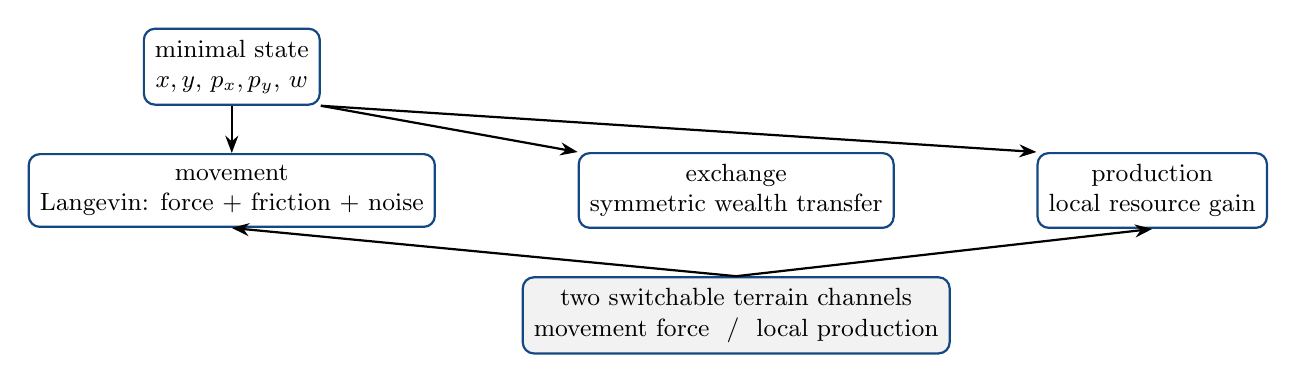
\begin{tikzpicture}[
  node distance=6mm and 7mm,
  box/.style={draw=accent, thick, rounded corners, minimum height=7mm, align=center, inner sep=4pt, font=\small},
  arr/.style={-{Stealth[length=2.2mm]}, thick},
]
  \node[box] (state) {minimal state\\ $x,y$, $p_x,p_y$, $w$};
  \node[box, below=of state] (move) {movement\\ Langevin: force $+$ friction $+$ noise};
  \node[box, right=18mm of move] (exch) {exchange\\ symmetric wealth transfer};
  \node[box, right=18mm of exch] (prod) {production\\ local resource gain};
  \draw[arr] (state.south) -- (move.north);
  \draw[arr] (state.south east) -- (exch.north west);
  \draw[arr] (state.south east) -- (prod.north west);
  \node[box, fill=black!5, below=of exch, align=center, font=\small] (ch) {two switchable terrain channels\\ movement force \ / \ local production};
  \draw[arr] (ch.north) -- (move.south);
  \draw[arr] (ch.north) -- (prod.south);
\end{tikzpicture}
\caption{\textbf{Model and intervention structure.} The landscape affects the
minimal state through exactly two switchable channels, making the causal
hypotheses falsifiable.}
\label{fig:model}
\end{figure}

\begin{figure}[t]
\centering
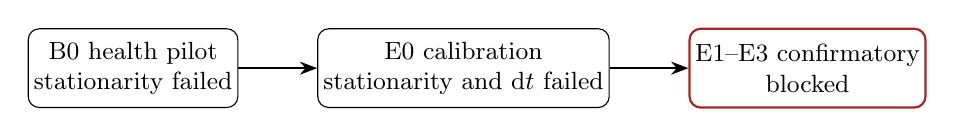
\begin{tikzpicture}[
  box/.style={draw, rounded corners, minimum width=24mm, minimum height=10mm, align=center, inner sep=2pt, font=\small},
  bad/.style={draw=warn, thick, rounded corners, minimum width=28mm, minimum height=10mm, align=center, inner sep=2pt, font=\small},
  okbox/.style={draw=ok, thick, rounded corners, minimum width=28mm, minimum height=10mm, align=center, inner sep=2pt, font=\small},
  arr/.style={-{Stealth[length=2.2mm]}, thick},
]
  \node[box] (b0) {B0 health pilot\\ stationarity failed};
  \node[box, right=10mm of b0] (e0) {E0 calibration\\ stationarity and $\mathrm{d}t$ failed};
  \node[bad, right=10mm of e0] (e1) {E1--E3 confirmatory\\ blocked};
  \draw[arr] (b0) -- (e0);
  \draw[arr] (e0) -- (e1);
\end{tikzpicture}
\caption{\textbf{Gate flow.} Executed health and calibration layers failed their
preregistered gates, so all confirmatory experiments were blocked before
outcomes were generated.}
\label{fig:gates}
\end{figure}

\section*{Methods}
\label{sec:methods}

\paragraph{Model.} Agent $i$ has state
$(x_i,y_i,p_{x,i},p_{y,i},w_i)$, with ability frozen to a constant in
Cycle 1 and population fixed. Positions and momenta follow a
Br\"unger--Brooks--Karplus Langevin update,
\begin{equation}
\mathrm{d}p = F\,\mathrm{d}t-\gamma p\,\mathrm{d}t+\sqrt{2\gamma m k_B T}\,\mathrm{d}W,
\qquad
\frac{\mathrm{d}x}{\mathrm{d}t}=\frac{p}{m},
\end{equation}
with $m=1$, friction $\gamma=1$, temperature $T=0.5$, and $k_B=1$. The
resource field $R(x,y)\ge0$ is converted to an elevation field
$H=R_{\max}-R$; the movement channel is a terrain force proportional to
$+\nabla R$ and the production channel is a local wealth gain
$R(x_i)\,\epsilon_i\,\mathrm{d}t$. The Cycle 1 landscape enters through only
these two switchable channels.

\paragraph{Wealth exchange.} Neighboring pairs within interaction range exchange
wealth through the label-symmetric, saturating rule
\begin{equation}
A_i=\epsilon_i\frac{w_i}{w_i+w_{\mathrm{ref}}},\qquad
\Delta w=\eta\frac{A_i-A_j}{A_i+A_j}\min(w_i,w_j),
\end{equation}
with exchange rate $\eta=0.003$ and half-saturation wealth $w_{\mathrm{ref}}=5$.
The transfer from $j$ to $i$ is zero-sum, so total wealth is conserved by
construction.

\paragraph{Landscape matching.} The clustered field is a mean-one field built
from five anisotropic Gaussian bumps with lognormal amplitudes; the shuffled
control is an exact pixel permutation, so total resources and the sorted
pixel histogram coincide by construction. A flat control equals the field mean.
An audit checks equal shape, exact sorted-histogram equality, non-negativity and
finiteness, and total-resource agreement within $10^{-12}$ relative tolerance.

\paragraph{Preregistration and analysis policy.} The primary observable is the
steady-window Spearman rank correlation between resource and binned population
density; co-primary observables are Moran's $I$ and occupancy entropy;
secondary observables include wealth Gini, wealth variance, total-wealth drift,
and effective sample size. Confirmatory effects were to be paired mean
differences with 10,000-sample bootstrap intervals and 100,000-sample paired
sign-flip $p$-values, with Holm correction. A simulation-resolution SESOI was
to be frozen from paired same-seed $\mathrm{d}t/2$ versus $\mathrm{d}t/4$
differences before any confirmatory outcome was inspected. In Cycle 1 this
gate failed, so no confirmatory effect was estimated.

\paragraph{Experiments.} \code{B0-DYNAMICS-PILOT} ran three seeds and passed
wealth non-negativity, fixed population, and finite-metric checks but failed
stationarity for all three seeds. \code{E0-NUMERICS} ran 5 seeds by 5
conditions (25 runs) and produced the calibration table above.
\code{E1-MATCHED-LANDSCAPES} (20 seeds by 4 conditions, $N=2000$,
$128\times128$), \code{E2-CHANNEL-ABLATION} (20 seeds by 2 landscapes by 4
channel states), and \code{E3-ROBUSTNESS-HOLDOUT} (populations, resolutions,
and held-out landscape families) were all blocked by upstream gates before any
confirmatory numeric artifact was produced.

\paragraph{Data availability.} All executed artifacts and blocked result files
are preserved under \code{research/jobs/<exp\_id>/}; the comprehensive record is
\code{research/paper/comprehensive/main.tex}. No new experiment was executed for
this journal draft.

\begin{thebibliography}{9}
\bibitem{duran2025}
M.~A.~Dur\'an-Olivencia, \emph{The Emergence of Socio-Economic Structure: A
First-Principles Kinetic Theory}, arXiv:2511.08742 (2025).
\bibitem{bae2026}
J.~Bae et al., \emph{Unveiling hidden features of social evolution by inferring
Langevin dynamics from data}, arXiv:2601.17772 (2026).
\bibitem{grimm2005}
V.~Grimm et al., Pattern-oriented modeling of agent-based complex systems:
lessons from ecology, \emph{Science} \textbf{310}, 987--991 (2005).
\bibitem{mcculloch2022}
J.~McCulloch et al., Uncertainty quantification for agent-based models,
\emph{J. Artif. Soc. Soc. Simul.} \textbf{25}(2), 1 (2022).
\end{thebibliography}

\end{document}
